\chapter{Training und Trainingszeit-Augmentierung}
\label{kap:trainingszeit}

\section{Aufbau}
\label{sec:trainingsaufbau}

\absatz{Datenaufteilung.} Trainiert wird auf synthetischen Bildern,
validiert auf dem \emph{realen} \code{val}-Bild (98 Objekte). Das ist eine
bewusste Entscheidung: Die Modellauswahl muss auf der Zieldomäne erfolgen, sonst
wählt man das Modell, das am besten zu den eigenen Renderartefakten passt.
\code{test} (89 Objekte) berührt Training und Modellauswahl nie und dient
ausschließlich der Endbewertung. Ein vierter Split \code{sval} aus 400
synthetischen Bildern mit anderem Seed dient allein der Messung des
Sim-to-Real-Abstands (Abschnitt~\ref{sec:simtoreal}).

\absatz{Zwei Budgets.} Die Arbeit trainiert Modelle in zwei Größenordnungen, und
es ist wichtig, sie nicht zu vermischen (Tabelle~\ref{tab:budgets}). Das
\textbf{Referenzmodell} nutzt den vollen Datensatz aus 6000 Bildern und
60~Epochen; es ist das Modell, dessen Zahlen als Ergebnis der Pipeline berichtet
werden (Abschnitt~\ref{sec:hauptergebnis}). Die \textbf{Ablationsarme} nutzen
jeweils 3000~Bilder und 30~Epochen. Dieses kleinere Budget ist eine Konzession an
die Rechenzeit -- mehrere Läufe statt einem --, und es ist \emph{für alle Arme
identisch}. Es begrenzt damit die absolute Höhe der Ablationszahlen, nicht ihren
Vergleich untereinander; Ablationszahlen sind deshalb ausschließlich mit
Ablationszahlen zu vergleichen, nie mit denen des Referenzmodells.

\begin{table}[htbp]
\centering
\caption[Die beiden Trainingsbudgets]{Die beiden Trainingsbudgets. Alles, was
nicht genannt ist, ist identisch: Architektur, Optimierer, Lernratenplan,
Verlustgewichte, Trainingszeit-Augmentierung, Seed, Validierungssplit.}
\label{tab:budgets}
\footnotesize
\begin{tabular}{@{}lcc@{}}
\toprule
 & \textbf{Referenzmodell} & \textbf{Ablationsarme (3$\times$)} \\
\midrule
Trainingsbilder & 6000 & 3000 \\
Epochenbudget & 60 (\code{patience}~20) & 30 (\code{patience}~20) \\
tatsächlich gelaufen & \zrefEpochen{} (bestes Modell: \zrefBestEpoche) & 30 \\
Batch & 8 & 8 \\
Bildzwischenspeicher & Festplatte & Festplatte \\
\bottomrule
\end{tabular}
\end{table}

Der Referenzlauf endete durch Early Stopping nach \zrefEpochen{} von
60~Epochen; das beste Modell stammt aus Epoche~\zrefBestEpoche. Die beiden
letzten Zeilen der Tabelle sind nicht gewählt, sondern erzwungen: \code{yolo26s-p2}
hält bei \code{imgsz}=1024 eine P2-Merkmalskarte mit $256\times256$ Zellen vor und
belegt bei Batch~16 rund 23,5\,GB -- alle Speicherangaben dieses Absatzes sind
mit \code{nvidia-smi} an den eigenen Läufen gemessen. Auf der verwendeten Karte waren zur Laufzeit
der Ablationen nur etwa 25\,GB frei; ein erster Lauf mit Batch~16 wich wiederholt
mit \code{CUDA OutOfMemoryError in TaskAlignedAssigner} auf die CPU aus -- was
nicht nur langsam ist, sondern die Läufe untereinander unvergleichbar macht, weil
der Ausweichpfad von der momentanen Fremdlast abhängt. Batch~8 belegt rund
13\,GB und läuft durchgängig auf der GPU.

\absatz{Modellwahl.} Durchgängig verwendet wird \code{yolo26s-p2} mit
9,66~Millionen Parametern (Modellzusammenfassung der Werkzeugkette,
Abschnitt~\ref{sec:p2kopf}). Die \emph{Größe} \enquote{s} folgt aus der Datenlage:
Der Datensatz hat eine Klasse und nur neun zugrunde liegende Objektinstanzen, die
Formvielfalt ist klein, die nötige Modellkapazität damit ebenfalls; die
\enquote{nano}-Variante verliert bei 12--40\px{} großen Objekten Rückruf, größere
Varianten würden die synthetischen Eigenheiten eher memorieren. Der \emph{P2-Kopf}
folgt aus der Auflösungsrechnung in Abschnitt~\ref{sec:p2kopf}: Er senkt die
Schrittweite der feinsten Detektionsebene von 8 auf 4 und die Zuweisungsgrenze
damit von 11,3 auf 5,7\px{} -- unter alle in \code{val} und \code{test}
auftretenden Objektgrößen. Er kostet dabei \emph{keine} Parameter (er hat 2,9\,\%
weniger als das Basismodell), sondern Speicher.

Ausgangspunkt sind COCO-vortrainierte Gewichte: Die vortrainierten
Low-Level-Filter sind domänenunabhängig \parencite{yosinski2014}, und
\textcite{hinterstoisser2018} zeigen den Nutzen explizit für synthetische
Trainingsdaten. Weil die \code{-p2}-Variante über eine Architekturdatei und nicht
über einen fertigen Checkpoint definiert ist, werden die Gewichte
\emph{partiell} übernommen: Backbone und die Ebenen P3--P5 aus \code{yolo26s.pt},
die zusätzlichen Blöcke der P2-Ebene zufällig initialisiert.

\absatz{Modellauswahl.} Gespeichert wird der Checkpoint mit der höchsten
Fitness auf dem realen \code{val}-Bild, wobei die Fitness der Werkzeugkette
$0{,}1 \cdot \mAPfifty + 0{,}9 \cdot \mAPall$ ist -- diese Gewichtung ist deren
Voreinstellung und wurde nicht verändert. Ein Detail ist dabei
festzuhalten: Diese Validierung läuft bei der \emph{Trainings}auflösung
\code{imgsz}=1024, während alle berichteten Zahlen bei nativem Maßstab (2464
bzw.\ 1600) gemessen werden. Auswahl- und Bewertungsauflösung fallen also
auseinander. Das ist hinnehmbar, weil die Rangfolge der Epochen von der
Auflösung kaum abhängt und die Alternative -- Auswahl bei nativem Maßstab --
eine zweite Validierung je Epoche kosten würde; es ist aber eine Annahme und
keine Messung, und sie gilt für alle Läufe gleich.

\absatz{Eingabegröße.} \code{imgsz}=1024, identisch zur Leinwandgröße des
Generators. Damit durchlaufen die synthetischen Bilder \emph{keine} Skalierung,
und die Objekte erreichen das Netz mit exakt der Pixelgröße, für die die Pipeline
ausgelegt ist (Anforderung~A2). Bei 640\px{} wären sie nach Gleichung~\eqref{eq:deff} nur noch 7--27\px{} groß
und lägen teils unter der Auflösung der P3-Ebene.

\absatz{Optimierung.} AdamW \parencite{loshchilov2019} mit
$\text{lr}_0 = 10^{-3}$, Endlernrate 1\,\% davon, Kosinusabfall
\parencite{loshchilov2017sgdr}, drei Aufwärmepochen, Weight Decay $5\cdot10^{-4}$,
Mixed Precision \parencite{micikevicius2018}, fester Seed und
deterministische Kernel. AdamW ist explizit gesetzt statt \code{auto}, weil es
bei kleinen Datensätzen schneller konvergiert und robust gegenüber der
Lernratenwahl ist -- wichtig, weil kein Budget für eine Lernratensuche vorhanden
ist. Die Verlustgewichte bleiben auf den Standardwerten
(\code{box}\,7,5 / \code{cls}\,0,5): Eine Erhöhung des Boxgewichts wäre bei
kleinen Objekten denkbar, ohne separaten Abstimmungssplit aber nicht belegbar.
Die Budgets stehen in Tabelle~\ref{tab:budgets}; Early Stopping greift jeweils
nach 20 Epochen ohne Verbesserung auf dem realen \code{val}-Bild. Bewusst
großzügig: Die Fitness schwankt auf knapp hundert Ground-Truth-Objekten stark,
ein knappes Fenster bräche zu früh ab.

\section{Augmentierungsparameter zur Trainingszeit}
\label{sec:trainparam}

Die abgeschalteten Parameter sind genauso begründungspflichtig wie die aktiven --
ein auf Null gesetzter Standardwert ist eine Entscheidung.

Aktiv sind Mosaic (immer, in den letzten zehn Epochen abgeschaltet), Skalierung
$0{,}6$--$1{,}4$, Translation, horizontale und vertikale Spiegelung sowie
HSV-Variation (Ton 0,015, Sättigung 0,7, Helligkeit 0,4). Abgeschaltet sind
\code{degrees}, \code{shear} und \code{perspective}, weil Bildrotation
achsparallele Boxen aufbläht -- bei $10^\circ$ um 15,8\,\% der Kantenlänge, was
die Überlappung mit der korrekten Box auf 0,745 senkt
(Abschnitt~\ref{sec:boxrotation}) --, sowie \code{mixup} und \code{cutmix}, die
Bildinhalte bei erhaltenen Labels überlagern und damit Geisterobjekte mit vollem
Boxlabel erzeugen \parencite{zhang2018mixup,yun2019cutmix}: Bei dicht gepackten
20\px-Objekten überwiegt der Labelkonflikt. \code{erasing} entfällt, weil es in
der Werkzeugkette nur bei der Klassifikation wirkt, und \code{copy\_paste},
weil es Segmentierungsmasken benötigt -- beides übernimmt der Generator
physikalisch korrekt. Die vollständige Tabelle mit Begründung je Parameter steht
im Anhang (Tabelle~\ref{tab:trainaug}).

Die beiden Augmentierungsschichten wirken bei der Objektgröße multiplikativ: Der
Generator erzeugt $[12, 44]$\px, die Trainingsskalierung multipliziert mit
$[0{,}6;\,1{,}4]$, sodass das Netz effektiv Objekte von
$12 \cdot 0{,}6 = 7{,}2$ bis $44 \cdot 1{,}4 = 61{,}6$\px{} sieht. Diese Spanne
deckt nach unten die Objektgrößen bei niedriger Inferenzauflösung und nach oben
jene bei starker Hochskalierung ab -- also den gesamten in
Abschnitt~\ref{sec:imgsz} durchmusterten Bereich. Sie deckt zugleich die vier
Objekte unter 12\px{} ab, die \code{test} enthält und die der Generator selbst
nicht erzeugt (Abschnitt~\ref{sec:valtest}). Der untere Rand von 7,2\px{} liegt
oberhalb der Zuweisungsgrenze $S\sqrt{2} = 5{,}7$\px{} der P2-Ebene, aber
\emph{unterhalb} der Grenze 11,3\px, die ohne P2-Kopf gälte: Erst die Modellwahl
aus Abschnitt~\ref{sec:p2kopf} macht \code{scale}$\,=0{,}4$ zu einem Wert, bei
dem auch der untere Rand der Trainingsverteilung noch zuverlässig zugewiesen
wird.

\section{Trainingsverlauf}
\label{sec:trainingsverlauf}

Abbildung~\ref{abb:training} zeigt die Lernkurven der drei Ablationsarme.
Drei Beobachtungen sind unabhängig vom Ausgang der Ablation.

\emph{Erstens} fällt der Trainingsverlust über alle 30 Epochen monoton, während
die Metrik auf dem realen \code{val}-Bild deutlich früher flach wird. Das ist der
Sim-to-Real-Abstand in zeitlicher Form: Ab dem Knick verbessert das Modell
überwiegend seine Anpassung an Eigenschaften der synthetischen Daten, die in der
Zieldomäne nicht gelten. Genau deshalb ist es methodisch notwendig, das beste
Modell über den \emph{realen} Validierungssplit auszuwählen; eine synthetische
Validierung wählte das Modell aus der letzten Epoche und damit das am stärksten
überangepasste.

\emph{Zweitens} liegt der Trainingsverlust des Arms mit dem naiven Verdecker
(B2) unter dem der beiden anderen, obwohl alle drei exakt dieselben Objekte an
denselben Stellen enthalten. Das ist für sich genommen kein Qualitätsurteil --
ein niedriger Trainingsverlust auf synthetischen Daten sagt nichts über die
Zieldomäne --, aber es zeigt, dass der Eingriff gewirkt hat: Ein flächig grauer
Verdecker macht dieselbe Szene messbar leichter.

\emph{Drittens} liegt die Kurve auf dem realen Bild deutlich unruhiger als der
Trainingsverlust. Das ist kein Trainingsproblem, sondern eine Folge der
Datenlage: Die Fitness wird an 98 Objekten \emph{eines} Bildes gemessen, und ein
einzelnes gefundenes oder verlorenes Objekt verschiebt den Rückruf bereits um
einen Prozentpunkt. Aus demselben Grund ist \code{patience} mit 20 Epochen
großzügig gesetzt -- ein knappes Fenster bräche bei dieser Streuung ab, bevor
das Modell auskonvergiert ist.

\begin{figure}[htbp]
\centering
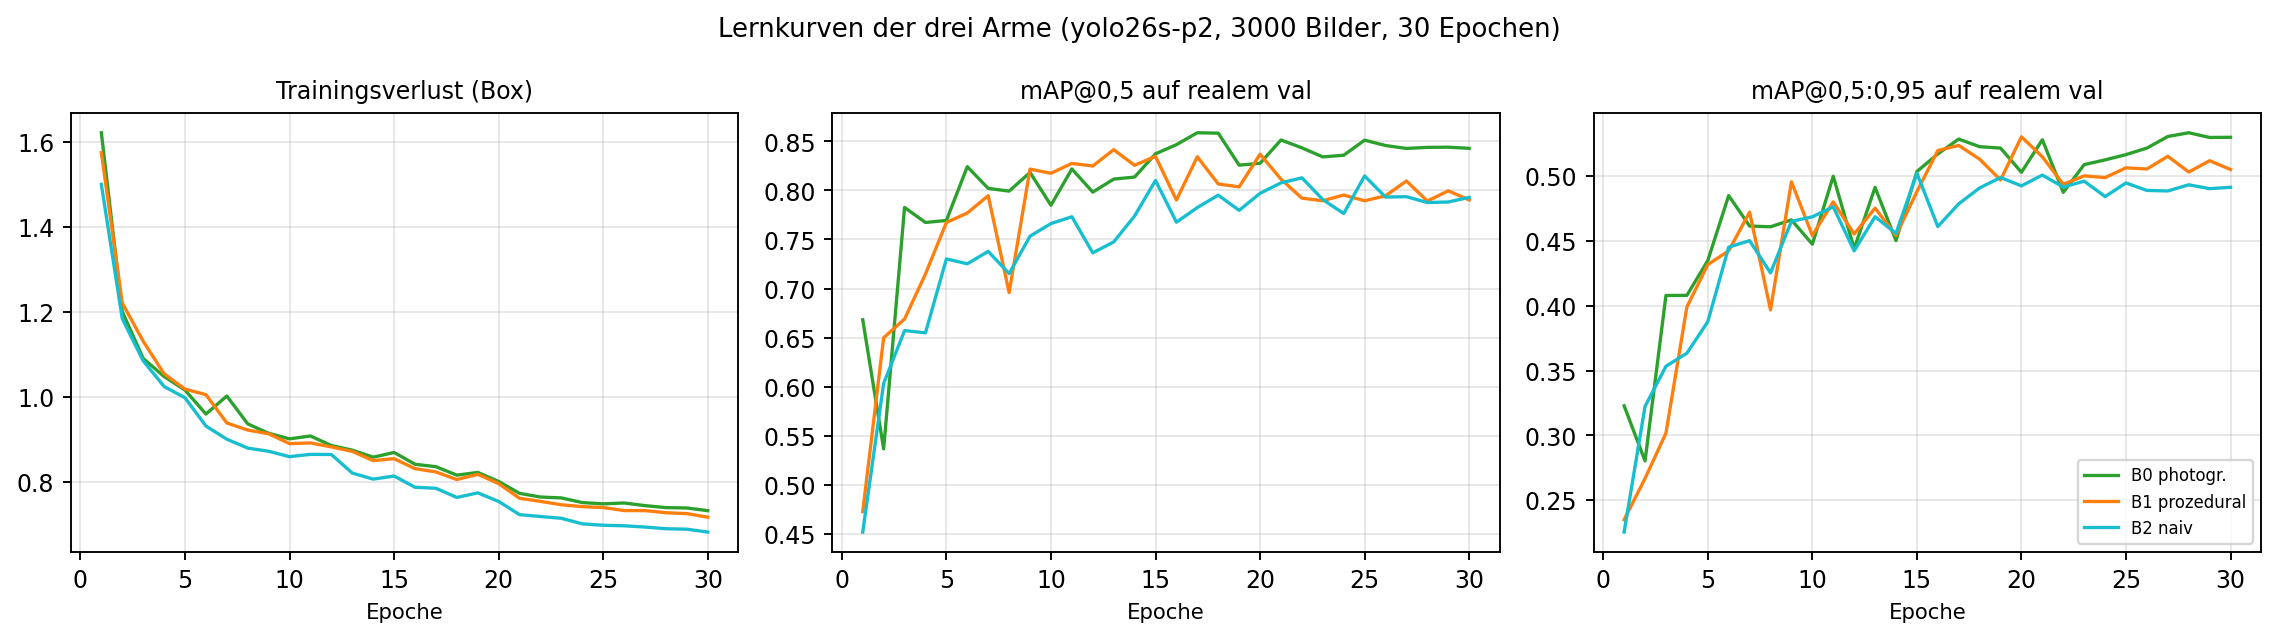
\includegraphics[width=\textwidth]{abbildungen/neu_training_b.png}
\caption[Lernkurven der Ablationsarme]{Lernkurven der drei Ablationsarme
(\code{yolo26s-p2}, 3000 Bilder, 30 Epochen, Batch~8). Links der
Box-Trainingsverlust auf den synthetischen Daten, Mitte und rechts \mAPfifty{}
und \mAPall{} auf dem realen \code{val}-Bild nach jeder Epoche. Diese
Validierung läuft bei der Trainingsauflösung \code{imgsz}=1024 und liegt
deshalb systematisch unter den in Kapitel~\ref{kap:auswertung} berichteten
Werten, die bei nativem Maßstab gemessen sind; für den \emph{Verlauf} ist das
ohne Belang. Der Knick
zwischen fallendem Verlust und flacher Realmetrik markiert den Punkt, ab dem
weiteres Training überwiegend synthetische Eigenheiten anpasst.}
\label{abb:training}
\end{figure}
